\addtocontents{toc}{\cftpagenumberson{part}}
\chapter*{APPENDIX SECTION}
\addcontentsline{toc}{part}{APPENDIX SECTION}
\label{ch:appendix}

% restarts the count of figures and tables
\renewcommand{\thetable}{A.\arabic{table}}  
\renewcommand{\thefigure}{A.\arabic{figure}}
\setcounter{figure}{0}
\setcounter{table}{0}

\begin{center}
APPENDIX A
\end{center}

\begin{figure}[ht]
\centering
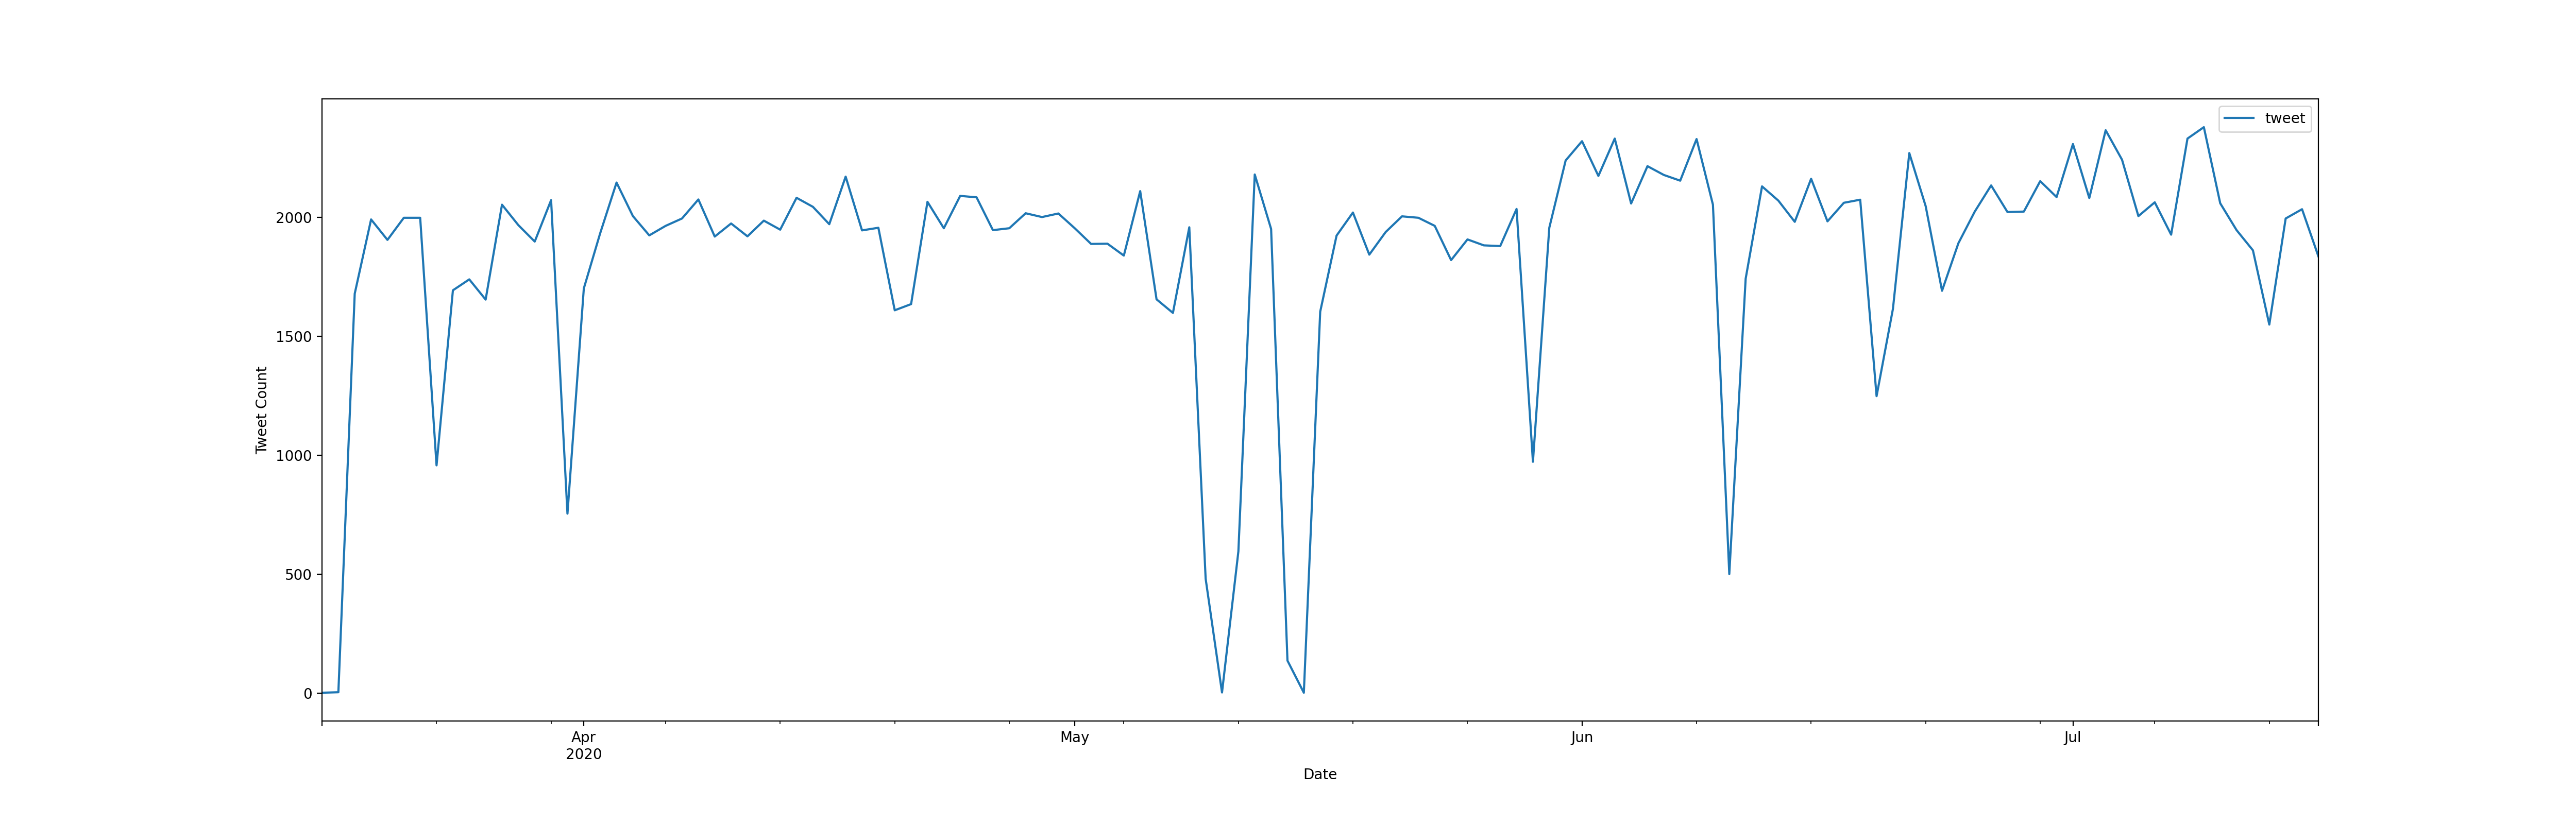
\includegraphics[scale=0.6]{Figs/Fig2.png}
\caption{First figure of appendix A. Captions of figures and tables in the Appendix section should not show up in the table of contents.}
\label{fig:figure1AP}
\end{figure}

\begin{table}[ht]
\caption{First table of appendix A. Captions of figures and tables in the Appendix section should not show up in the table of contents.}
\centering
\fontsize{10}{12}\selectfont
\begin{tabular}{|l|r|r|}
\hline
Dataset name & Number of records  & Number of users \\
\hline 
Dataset A & 248 & 20 \\
\hline
Dataset B & 464 & 28 \\
\hline
Dataset C & 348 & 7 \\
\hline
Dataset D & 419 & 5\\
\hline
Dataset E & 854 & 15\\
\hline
\end{tabular}
\label{tab:table1AP}
\end{table}


\begin{table}[ht]
\caption{Second table of appendix A. Captions of figures and tables in the Appendix section should not show up in the table of contents.}
\centering
\fontsize{10}{12}\selectfont
\begin{tabular}{|l|r|r|}
\hline
Dataset name & Number of records  & Number of users \\
\hline 
Dataset F & 1000 & 10 \\
\hline
Dataset G & 2000 & 20 \\
\hline
Dataset H & 3000 & 30 \\
\hline
Dataset I & 4000 & 40\\
\hline
Dataset J & 5000 & 50\\
\hline
\end{tabular}
\label{tab:table2AP}
\end{table}



\clearpage
\pagebreak


% restarts the count of figures and tables
\renewcommand{\thetable}{B.\arabic{table}}  
\renewcommand{\thefigure}{B.\arabic{figure}}
\setcounter{figure}{0}
\setcounter{table}{0}


\FloatBarrier
\begin{center}
APPENDIX B
\end{center}


\begin{table}[ht]
\caption{First table of appendix B. Captions of figures and tables in the Appendix section should not show up in the table of contents.}
\centering
\fontsize{10}{12}\selectfont
\begin{tabular}{|l|r|r|}
\hline
Column 1 & Column 2  & Column 3 \\
\hline 
1 & 2 & 10000 \\
\hline
3 & 4 & 20000 \\
\hline
5 & 6 & 30000 \\
\hline
\end{tabular}
\label{tab:table3AP}
\end{table}


\begin{table}[ht]
\caption{Second figure of appendix B. Captions of figures and tables in the Appendix section should not show up in the table of contents.}
\centering
\fontsize{10}{12}\selectfont
\begin{tabular}{|l|r|r|}
\hline
Column 1 & Column 2  & Column 3 \\
\hline 
A & B & 10000 \\
\hline
C & D & 20000 \\
\hline
E & F & 30000 \\
\hline
\end{tabular}
\label{tab:table4AP}
\end{table}


\begin{figure}[ht]
\centering
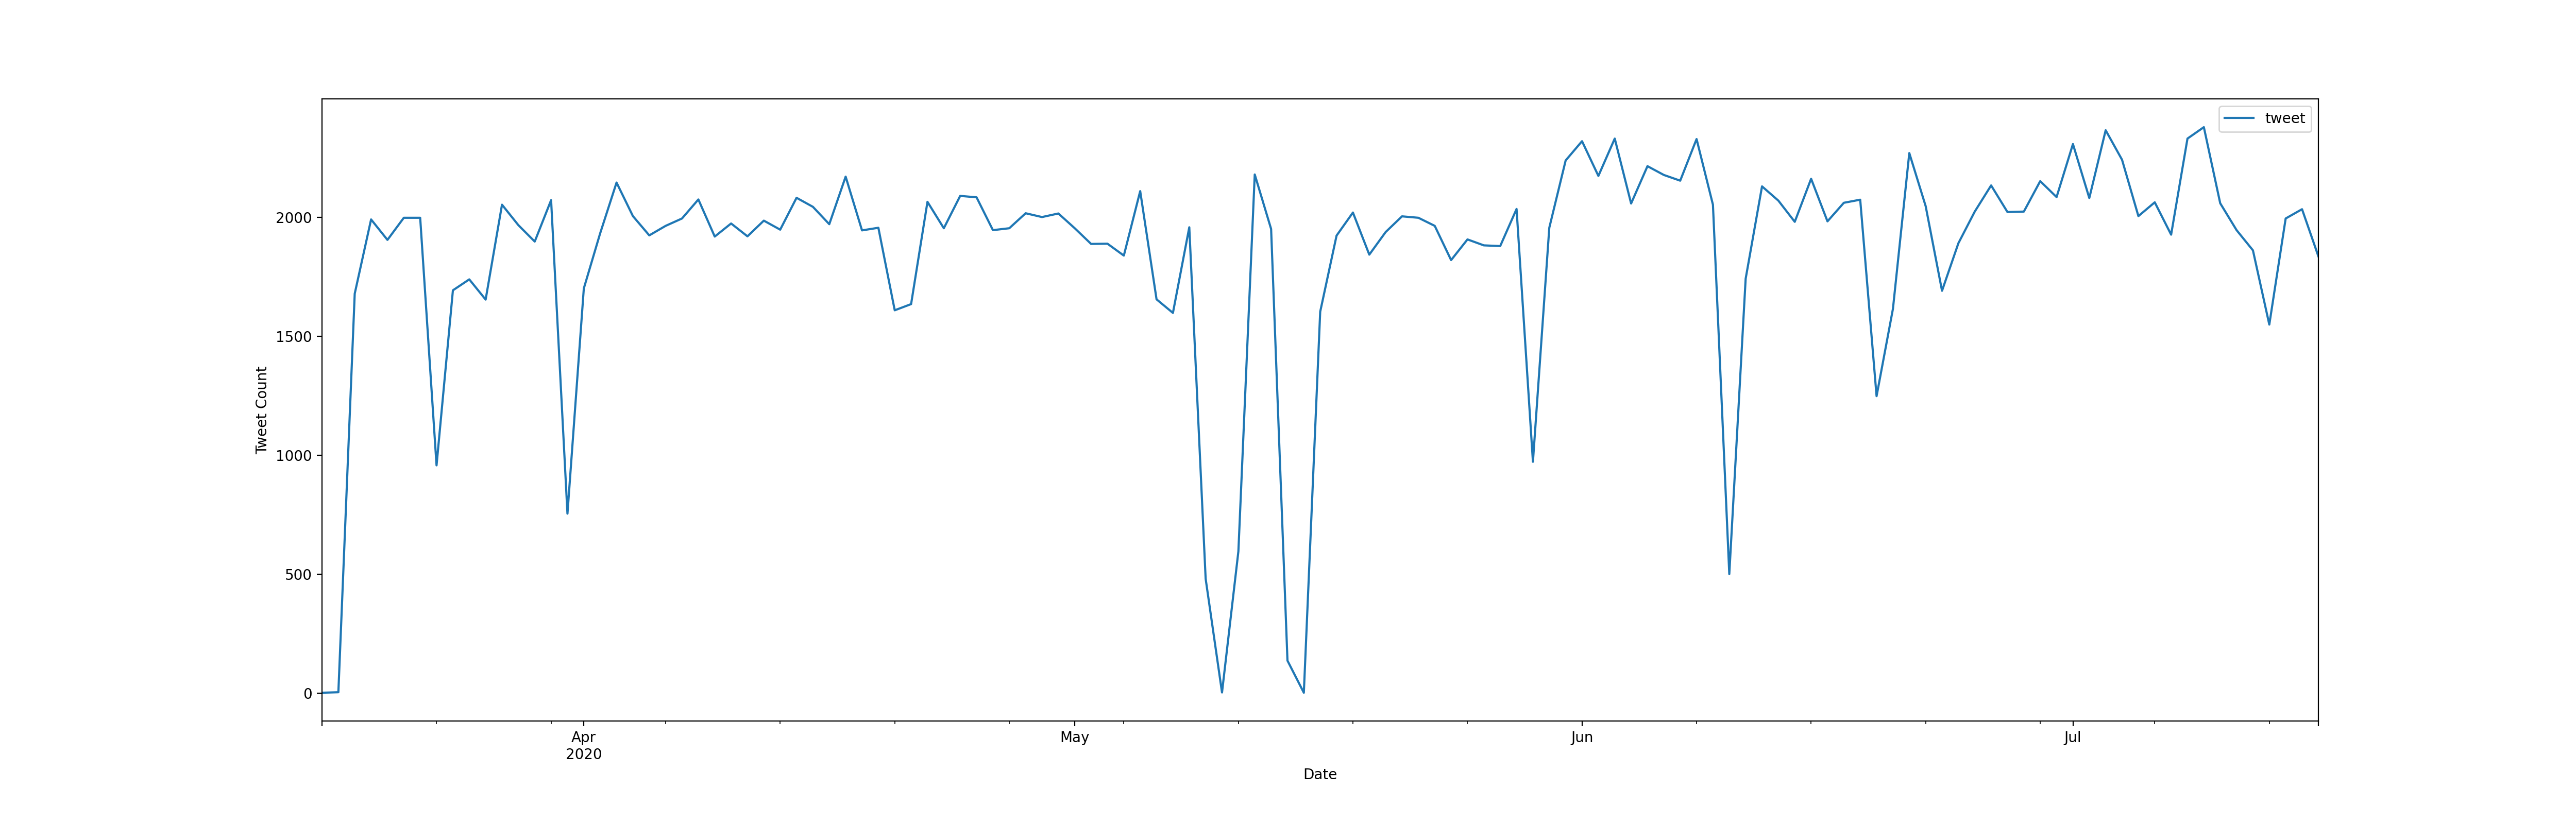
\includegraphics[scale=0.22]{Figs/Fig2.png}
\caption{First figure of appendix B. Captions of figures and tables in the Appendix section should not show up in the table of contents.}
\label{fig:figure3AP}
\end{figure}



